% Elsevier single-column paper using the teacher-supplied elsarticle bundle.
% Compiler: pdfLaTeX. Body English is retained from the edited Word source.
\documentclass[final,3p,12pt,nopreprintline]{elsarticle}
\usepackage[T1]{fontenc}
\usepackage{lmodern}
\usepackage[utf8]{inputenc}
\usepackage{amsmath,amssymb}
\usepackage{booktabs,array,tabularx,multirow}
\usepackage{graphicx,rotating,adjustbox}
\usepackage{xurl}
\usepackage[hidelinks]{hyperref}
\usepackage{microtype}
\graphicspath{{figures/}}
\DeclareGraphicsExtensions{.pdf,.png,.jpeg,.jpg}
\hyphenation{data-center work-load infra-struc-ture accel-er-ator repro-duc-ible}
\newcommand{\framework}{WISP-DC}
\newcommand{\ttft}{\mathrm{TTFT}}
\newcommand{\tpot}{\mathrm{TPOT}}
\emergencystretch=1.5em
\renewcommand{\topfraction}{0.95}
\renewcommand{\bottomfraction}{0.9}
\renewcommand{\textfraction}{0.05}
\renewcommand{\floatpagefraction}{0.75}
\makeatletter
\let\ps@pprintTitle\ps@plain
\makeatother
\pagestyle{plain}
\begin{document}
\begin{frontmatter}
\title{WISP-DC: A Benchmark-Trace-Based Feasibility Framework for Workload-Specific AI Infrastructure Planning}
\author{Raazia Imran Reshamwala}
\author{Syed Muhammad Sheraz}
\author{Maham Faisal}
\begin{abstract}Setting an AI-capable data center and high performance compute farm demands an early infrastructure decision: which available configuration can handle a defined workload without breaking performance and resource limits? The outcome hinges on the workload. Training is controlled by time-to-quality, whereas online inference must balance throughput, tail-latency, and accuracy conditions simultaneously. This paper details WISP-DC, an explainable feasibility framework that splits empirical performance proof from planning assumptions and ranks only configurations that pass every declared hard constraint. The framework was validated through two replicable, trace-driven scenarios. Scenario 1 used 30 raw MLPerf Training v4.0 ResNet-50 logs covering six H100 configurations from 4 to 64 accelerators. Depending on the deadline, the minimum-accelerator recommendation shifted across 4 to 8, 16, or 64 GPUs; no tested system met a two-minute deadline. Scenario 2 used four MLPerf Inference v5.0 Llama 2 70B Server results. Six predefined cases detailed that 4,000 and 8,000 output tokens/s were feasible with one and two GH200 accelerators, respectively; 20,000 tokens/s was infeasible under a two-accelerator ceiling but feasible with eight H100 accelerators; and 32,000 tokens/s exceeded every evaluated result. After excluding three price-dependent tests for which the underlying regional rate could not be separately logged, the preserved implementations passed 24 evidence-supported automated checks and executed 99 inference sensitivity cases. Power, rack, and energy calculations are reported only where their evidence boundary is met; financial optimization is not claimed. The study simply authenticates the framework’s decision logic, rather than claiming new execution speeds or whole data center layout specifications.\end{abstract}
\begin{keyword}AI infrastructure, capacity planning, feasibility analysis, MLPerf, workload-aware systems, training, inference, explainable decision support.\end{keyword}
\end{frontmatter}

\section{Introduction}


% Word blocks 11,12; 1 Introduction, paragraph 1
AARTIFICIAL-INTELLIGENCE platforms concentrate massive processing power within a compact physical footprint. This makes the initial scoping strategy crucial: a con-figuration that is insufficient fails to meet the service target, whereas one that is excessively ample squanders limited accelerators and may create avoidable power, space and cost overheads. The International Energy Agency forecasts global data-center electricity utilization to increase to roughly 945 TWh by 2030 in its base case, with accelerated servers accounting for a significant fraction of the increase \hyperref[ref:1]{[1]}. Earlier global analysis also showed why simple proportional extrapolation is flawed: demand can expand while enhancements in hardware, software, and utilization moderate energy growth \hyperref[ref:2]{[2]}. In other words, infrastructure should be sized from the work it must deliver, not from a generic label such as “AI server.”


% Word blocks 13,18; 1 Introduction, paragraph 2
Training and inference intensify this arbitration in dif-ferent paradigms. A training system must reach a precison target before a deadline. Adding accelerators can shorten the run, but the gain need not be linear and the larger system can impose a higher instantaneous power envelope. An online inference system instead faces a parallel set of requirements: request throughput, time to first token, time per output token, quality, and a allocation threshould. A high-throughput result is not useful if it breaches the latency or accuracy condition. Production traces likewise show that large-model development has heterogeneous job dynamics and non-trivial resource-utilization constraints \hyperref[ref:3]{[3]}.


% Word blocks 19,20; 1 Introduction, paragraph 3
Published evaluations provide a practical empirical basis for feasibility studies when the researchers do not own dozens of current accelerators. MLPerf Training re-ports time-to-quality under a regulated benchmark protocol \hyperref[ref:4]{[4]}; MLPerf Inference assesses performance under defined deployment scenarios and quality rules \hyperref[ref:5]{[5]}. Yet a benchmark table does not answer a user’s provisioning question by itself. The table must be screened by the user’s constraints, alterna-tives must be ranked under an explicit rule, and the outcome must explain why each candidate passed or failed.


% Word blocks 21; 1 Introduction, paragraph 4
This paper proposes and evaluates WISP-DC, a rule-based, workload-first feasibility framework. It does not purport to train ResNet-50 or execute Llama 2 70B locally. Instead, it treats official MLPerf records as empirical logs and evaluates the planning logic around those records. The present study explores three research questions:


\begin{itemize}

\item RQ1: Can a single architecture express the different hard constraints needed for AI training and online inference?

\item RQ2: Does the implemented decision logic return the minimum-resource feasible evaluated configuration, and a justified infeasible result when no candidate passes?

\item RQ3: Which conclusions remain valid when per-formance evidence, engineering proxies, prices, and scenario assumptions are kept separate?

\end{itemize}

% Word blocks 27; 1 Introduction, paragraph 5
The paper details four specific points. First, it maps out an verifable workload-to-configuration process that decouples hard-constraint filtering from scoring. Second, it incorporates separate training and inference decision models without extrapolating  performance for unverified systems. Third, it gives a reproducible evaluation artifact comprising source records, scenario inputs, generated outputs, manual checks, sensitivity cases, and automated tests. Fourth, it shows how rack, energy, heat, and cost information can be integrated without presenting a surrogate as a physical measurement. The evaluated purview is AI training and online AI inference retrofitting, return on investment, cooling infrastructure, and broad HPC or enterprise-workload verification are omitted.


% Word blocks 28; 1 Introduction, paragraph 6
The rest of the paper examines related work, defines the framework and evidence boundary, describes the experiments, presents the results, and discusses validity andoperational impacts.


\section{Related Work}


\subsection{Energy and Capacity Planning}


% Word blocks 32; 2.1 Energy and Capacity Planning, paragraph 1
Data-center energy research spans component models, server models, network models, and whole-facility models. Dayarathna et al. survey these levels and emphasize that model selection depends on the purpose of the analysis \hyperref[ref:6]{[6]}. Fan et al. show that the sum of nameplate ratings is not nec-essarily an accurate representation of attainable aggregate demand, although rated values remain useful for conserva-tive electrical planning \hyperref[ref:7]{[7]}. These distinctions are especially important for accelerator-dense systems: operational energy, expected peak demand, and installed electrical capacity are different quantities.


% Word blocks 33; 2.1 Energy and Capacity Planning, paragraph 2
Recent measurement work reinforces that point. Latif et al. measure an eight-H100 node during ResNet and Llama 2 training and report workload-specific demand be-low the rated node limit \hyperref[ref:8]{[8]}. Vercellino et al. provide high-resolution profiles for generative-AI training, fine-tuning, and inference to support facility planning \hyperref[ref:9]{[9]}. Such measure-ments can calibrate preliminary estimates, but transferring a value between non-identical systems introduces uncertainty. WISP-DC therefore labels each numerical field as measured benchmark evidence, vendor evidence, derived output, or declared assumption.


\subsection{AI Benchmarks and Workload Characterization}


% Word blocks 36; 2.2 AI Benchmarks and Workload Characterization, paragraph 1
MLPerf Training uses an end-to-end time-to-quality objec-tive, which is more suitable for training feasibility than raw samples per second alone \hyperref[ref:4]{[4]}. MLPerf Inference defines deployment scenarios, performance metrics, and accuracy requirements so that systems can be compared under a com-mon workload definition \hyperref[ref:5]{[5]}. The official v4.0 Training and v5.0 Inference repositories retain system disclosures, result logs, and implementation records \hyperref[ref:10]{[10]}, \hyperref[ref:11]{[11]}. This provenance makes the records suitable for a trace-replay study.


% Word blocks 37,38; 2.2 AI Benchmarks and Workload Characterization, paragraph 2
Standardization does not eliminate context. Performance remains tied to the model, dataset, precision, software stack, benchmark version, and submitted hardware. Nor does a published score determine which system should be pur-chased: the answer depends on the user’s demand and resource limits. WISP-DC treats a benchmark result as an observed point, not as a universal scaling coefficient.


\subsection{Resource Management and the Remaining Plan-ning Gap}


% Word blocks 41; 2.3 Resource Management and the Remaining Plan-ning Gap, paragraph 1
Energy-aware allocation studies have largely focused on runtime management. Beloglazov et al. propose consol-idation heuristics that reduce energy while maintaining service constraints \hyperref[ref:12]{[12]}. GreenCloud provides packet-level simulation of servers, switches, links, and workloads \hyperref[ref:13]{[13]}. Thermal-aware placement shows that workload scheduling and temperature cannot always be separated \hyperref[ref:14]{[14]}. These studies are valuable once a data center and its resources exist.


% Word blocks 42; 2.3 Resource Management and the Remaining Plan-ning Gap, paragraph 2
The question studied here occurs earlier: given a specific AI workload and a finite catalogue of evidenced systems, which candidates are technically feasible, which candidate is preferred under a declared ranking rule, and why? Ta-ble 1 positions this contribution. The novelty is not a new benchmark or power model; it is the traceable combination of workload-specific feasibility rules, evidence boundaries, and reproducibility checks.


\subsection{Sustainable Planning and Decision Transparency}


% Word blocks 45; 2.4 Sustainable Planning and Decision Transparency, paragraph 1
Sustainable data-center planning is broader than lowering one power value. Shuja et al. organize energy-efficient data-center techniques across computing infrastructure, resource management, thermal behavior, and energy supply \hyperref[ref:15]{[15]}. Carbon Explorer similarly demonstrates that operational choices, embodied impacts, power sources, and system life-time can lead to different design conclusions \hyperref[ref:16]{[16]}. These studies are a useful warning against converting a single benchmark score into a broad sustainability claim. The present work therefore uses the term feasibility in a precise sense: satisfaction of declared performance and resource constraints within the available evidence. Energy and cost are attached as secondary decision attributes only when comparable inputs exist.


% Word blocks 46; 2.4 Sustainable Planning and Decision Transparency, paragraph 2
Explainability is equally important because an infra-structure recommendation can fail for several unrelated reasons. A configuration may lack sufficient throughput, exceed the allowed accelerator count, miss a latency target, fail the required accuracy threshold, or violate an applicable rack or budget limit. A single composite score can conceal such a failure. WISP-DC instead keeps a Boolean pass/fail record for every hard constraint and exposes the ranking rule used after filtering. This design favors auditability over an opaque weighted score.


\subsection{Evidence Reuse as an Evaluation Method}


% Word blocks 49,51; 2.5 Evidence Reuse as an Evaluation Method, paragraph 1
Trace-driven evaluation is appropriate when a research con-tribution concerns a decision process rather than a new hardware or learning algorithm. It allows the same evi-dence to be replayed under different requirements, makes boundary cases repeatable, and separates errors in source extraction from errors in recommendation logic. Its principal weakness is dependence on the external experiment: the researcher can verify the mapping applied to the trace but cannot purport to have independently reproduced the physical measurement. This paper incorporates that limita-tion unambiguously. The MLPerf logs are empirical inputs, and every claim about WISP-DC is confined to what the implemented transformations and tests establish.


\begin{table}[htbp]
\caption{Positioning of \framework{} Relative to Representative Work}
\label{tab:positioning}
\centering
\footnotesize
\setlength{\tabcolsep}{3pt}
\renewcommand{\arraystretch}{1.12}
\begin{tabularx}{\textwidth}{p{2.8cm}XXXX}
\toprule
\textbf{Work} & \textbf{Primary purpose} & \textbf{Workload evidence} & \textbf{Planning decision} & \textbf{Validation form} \\
\midrule
MLPerf Training \hyperref[ref:4]{[4]} & Standardized training comparison & Time-to-quality & No user-specific selection & Controlled benchmark \\
MLPerf Inference \hyperref[ref:5]{[5]} & Standardized inference comparison & Throughput, latency, accuracy & No user-specific selection & Controlled benchmark \\
Beloglazov \emph{et al.} \hyperref[ref:12]{[12]} & Runtime consolidation & Simulated cloud demand & VM allocation & Simulation \\
GreenCloud \hyperref[ref:13]{[13]} & Energy-aware network simulation & Configurable workloads & Simulated allocation/topology & Packet-level simulation \\
Latif \emph{et al.} \hyperref[ref:8]{[8]} & AI-node power characterization & Measured H100 node & No infrastructure recommendation & Physical measurement \\
Proposed \framework{} & Early feasibility decision & Published MLPerf traces & Recommend an evidenced candidate or return infeasible & Source reconciliation, cases, tests, sensitivity \\
\bottomrule
\end{tabularx}
\end{table}

\section{Framework and Method}


\subsection{Scope and Evidence Boundary}


% Word blocks 55; 3.1 Scope and Evidence Boundary, paragraph 1
WISP-DC acts as a simple checking step between what a user needs and a list of eligible systems. It answers a very specific question: does a tested setup meet every strict rule, and if a few do, which one does the standard tie-breaker choose? The tool never makes up an unseen cluster on the fly, guesses performance using flat scaling lines, or takes the place of official electrical, weight, and cooling blueprints "WISP-DC acts as a simple checking step between what a user needs and a list of eligible systems. It answers a very specific question: does a tested setup meet every strict rule, and if a few do, which one does the standard tie-breaker choose? The tool never makes up an unseen cluster on the fly, guesses performance using flat scaling lines, or takes the place of official electrical, weight, and cooling blueprints


% Word blocks 56; 3.1 Scope and Evidence Boundary, paragraph 2
The evidence ledger uses four classes:


\begin{enumerate}

\item empirical benchmark evidence: MLPerf timestamps, throughput, latency, accuracy, and submitted sys-tem descriptions;

\item vendor evidence: form factor, weight, device memory, and conservative electrical specifications;

\item derived outputs: differences, trimmed means, feasi-bility flags, energy arithmetic, and heat conversion; and

\item scenario assumptions: deadlines, accelerator ceilings, PUE, rack limits, and run frequency.

\end{enumerate}

% Word blocks 61; 3.1 Scope and Evidence Boundary, paragraph 3
Empty data simply stays empty. For instance, the four-GPU training choice is still kept for the speed sorting step even though a matching server power number was not there; the code simply skips running power calculations for it. The hardware cross-checks follow the same rule. NVIDIA’s H100 specification is used as a device-rating refer-ence \hyperref[ref:17]{[17]}, while the Dell XE9680 rack-integration guide and HPE XD670 QuickSpecs support model-specific physical and conservative electrical fields \hyperref[ref:18]{[18]}, \hyperref[ref:19]{[19]}. These documents do not substitute for workload performance or whole-system energy measurements.


\subsection{Architecture}


% Word blocks 75,76,81,90,62; 3.2 Architecture, paragraph 1
Figure 1 presents the evaluated decision path. The user input becomes a scenario-specific workload profile. The training or inference model then filters empirical candidates. A feasible set is ranked; an empty set produces an explicit infeasible outcome. Supporting rack, power-proxy, and cost checks are added only when their data boundary is satisfied. The prototype documentation also contains broader ta-bles for servers, GPUs, CPUs, storage, networking, racks, PDUs, UPS equipment, cooling-related hardware, and power distribution. These tables are valuable for implement-ing a future catalogue service, but they were not used as performance evidence in S1 or S2. Several are heterogeneous compilations rather than analysis-ready relational tables, two uploaded power-distribution files are duplicates, and some fields are estimates or “not stated.” In the present paper, only matching OEM server/GPU facts support static cross-checks. The broader catalogue is therefore shown as a separate prototype layer rather than merged with the experimental dataset.


\begin{figure}[htbp]
  \centering
  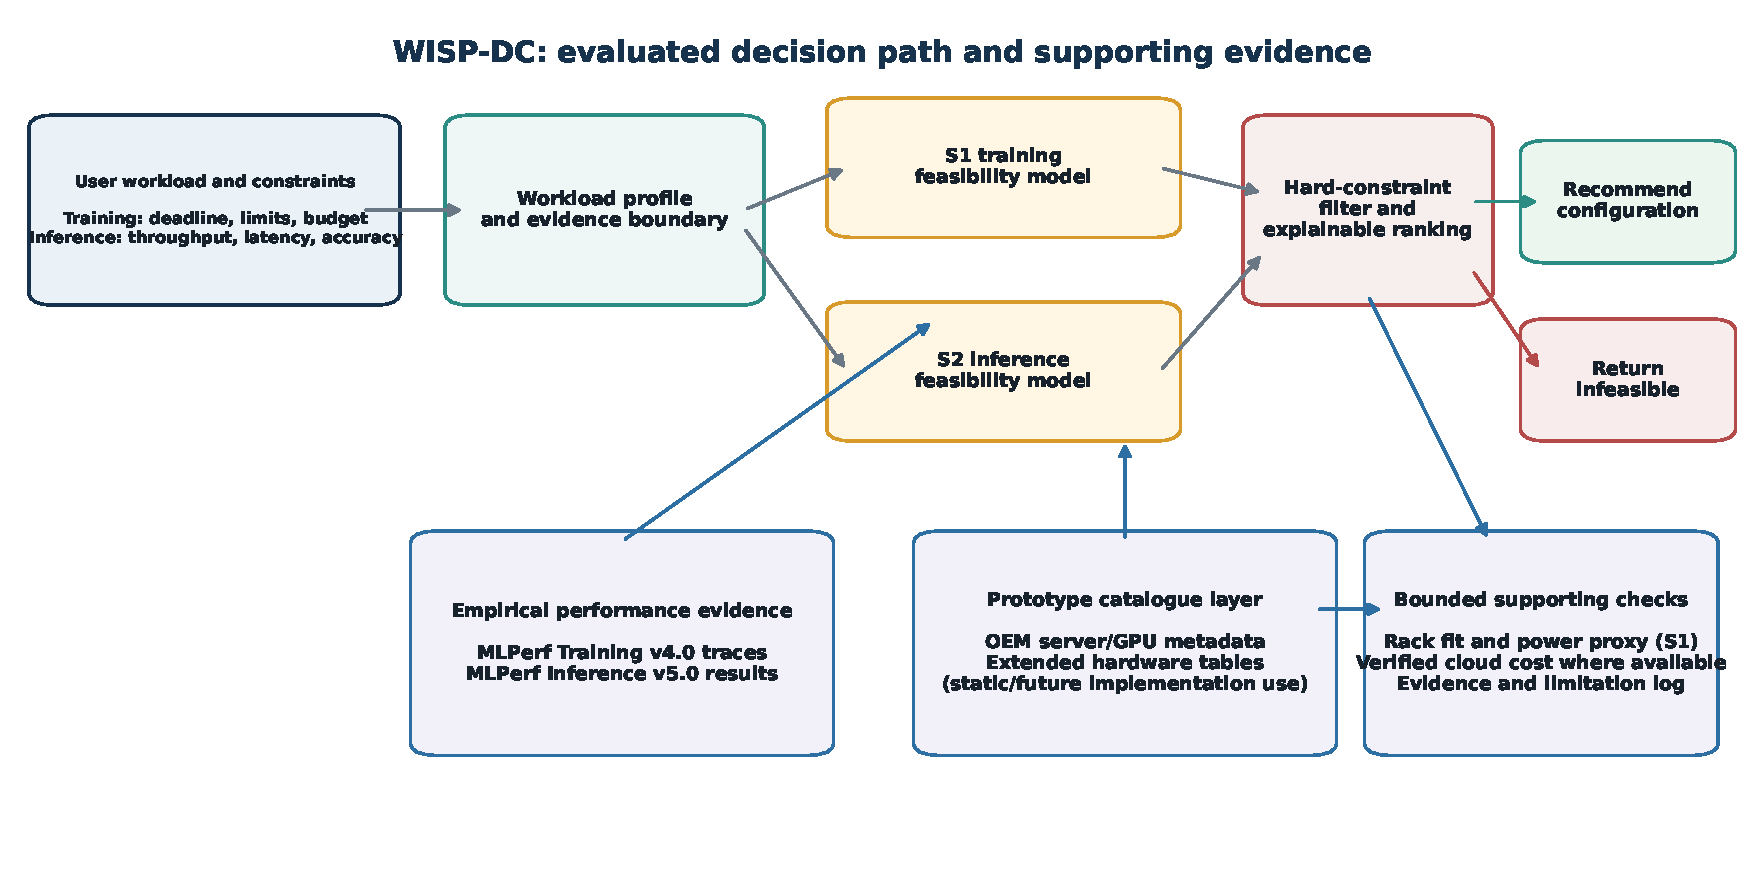
\includegraphics[width=\textwidth]{wisp_dc_architecture.pdf}
  \caption{WISP-DC architecture. Solid decision stages were evaluated through S1 and S2. The broader prototype catalogue is documented separately and is not presented as benchmark validation.}
  \label{fig:architecture}
\end{figure}

% Word blocks 63; 3.2 Architecture, paragraph 2
The evaluated path in Fig. 1 sits within a broader archi-tecture proposed for the full prototype. Figure 2 shows how workload profiling, infrastructure sizing, energy, cost, risk, existing-facility assessment, evidence sources, and reporting are intended to interact. It is included as a conceptual system map rather than an implementation claim. The present experiments exercise only the S1 and S2 feasibility path described in this paper; the existing-facility workflow, com-plete cost and cooling engines, external interfaces, and ex-tended reporting functions remain future prototype scope.


\begin{sidewaysfigure}[p]
  \centering
  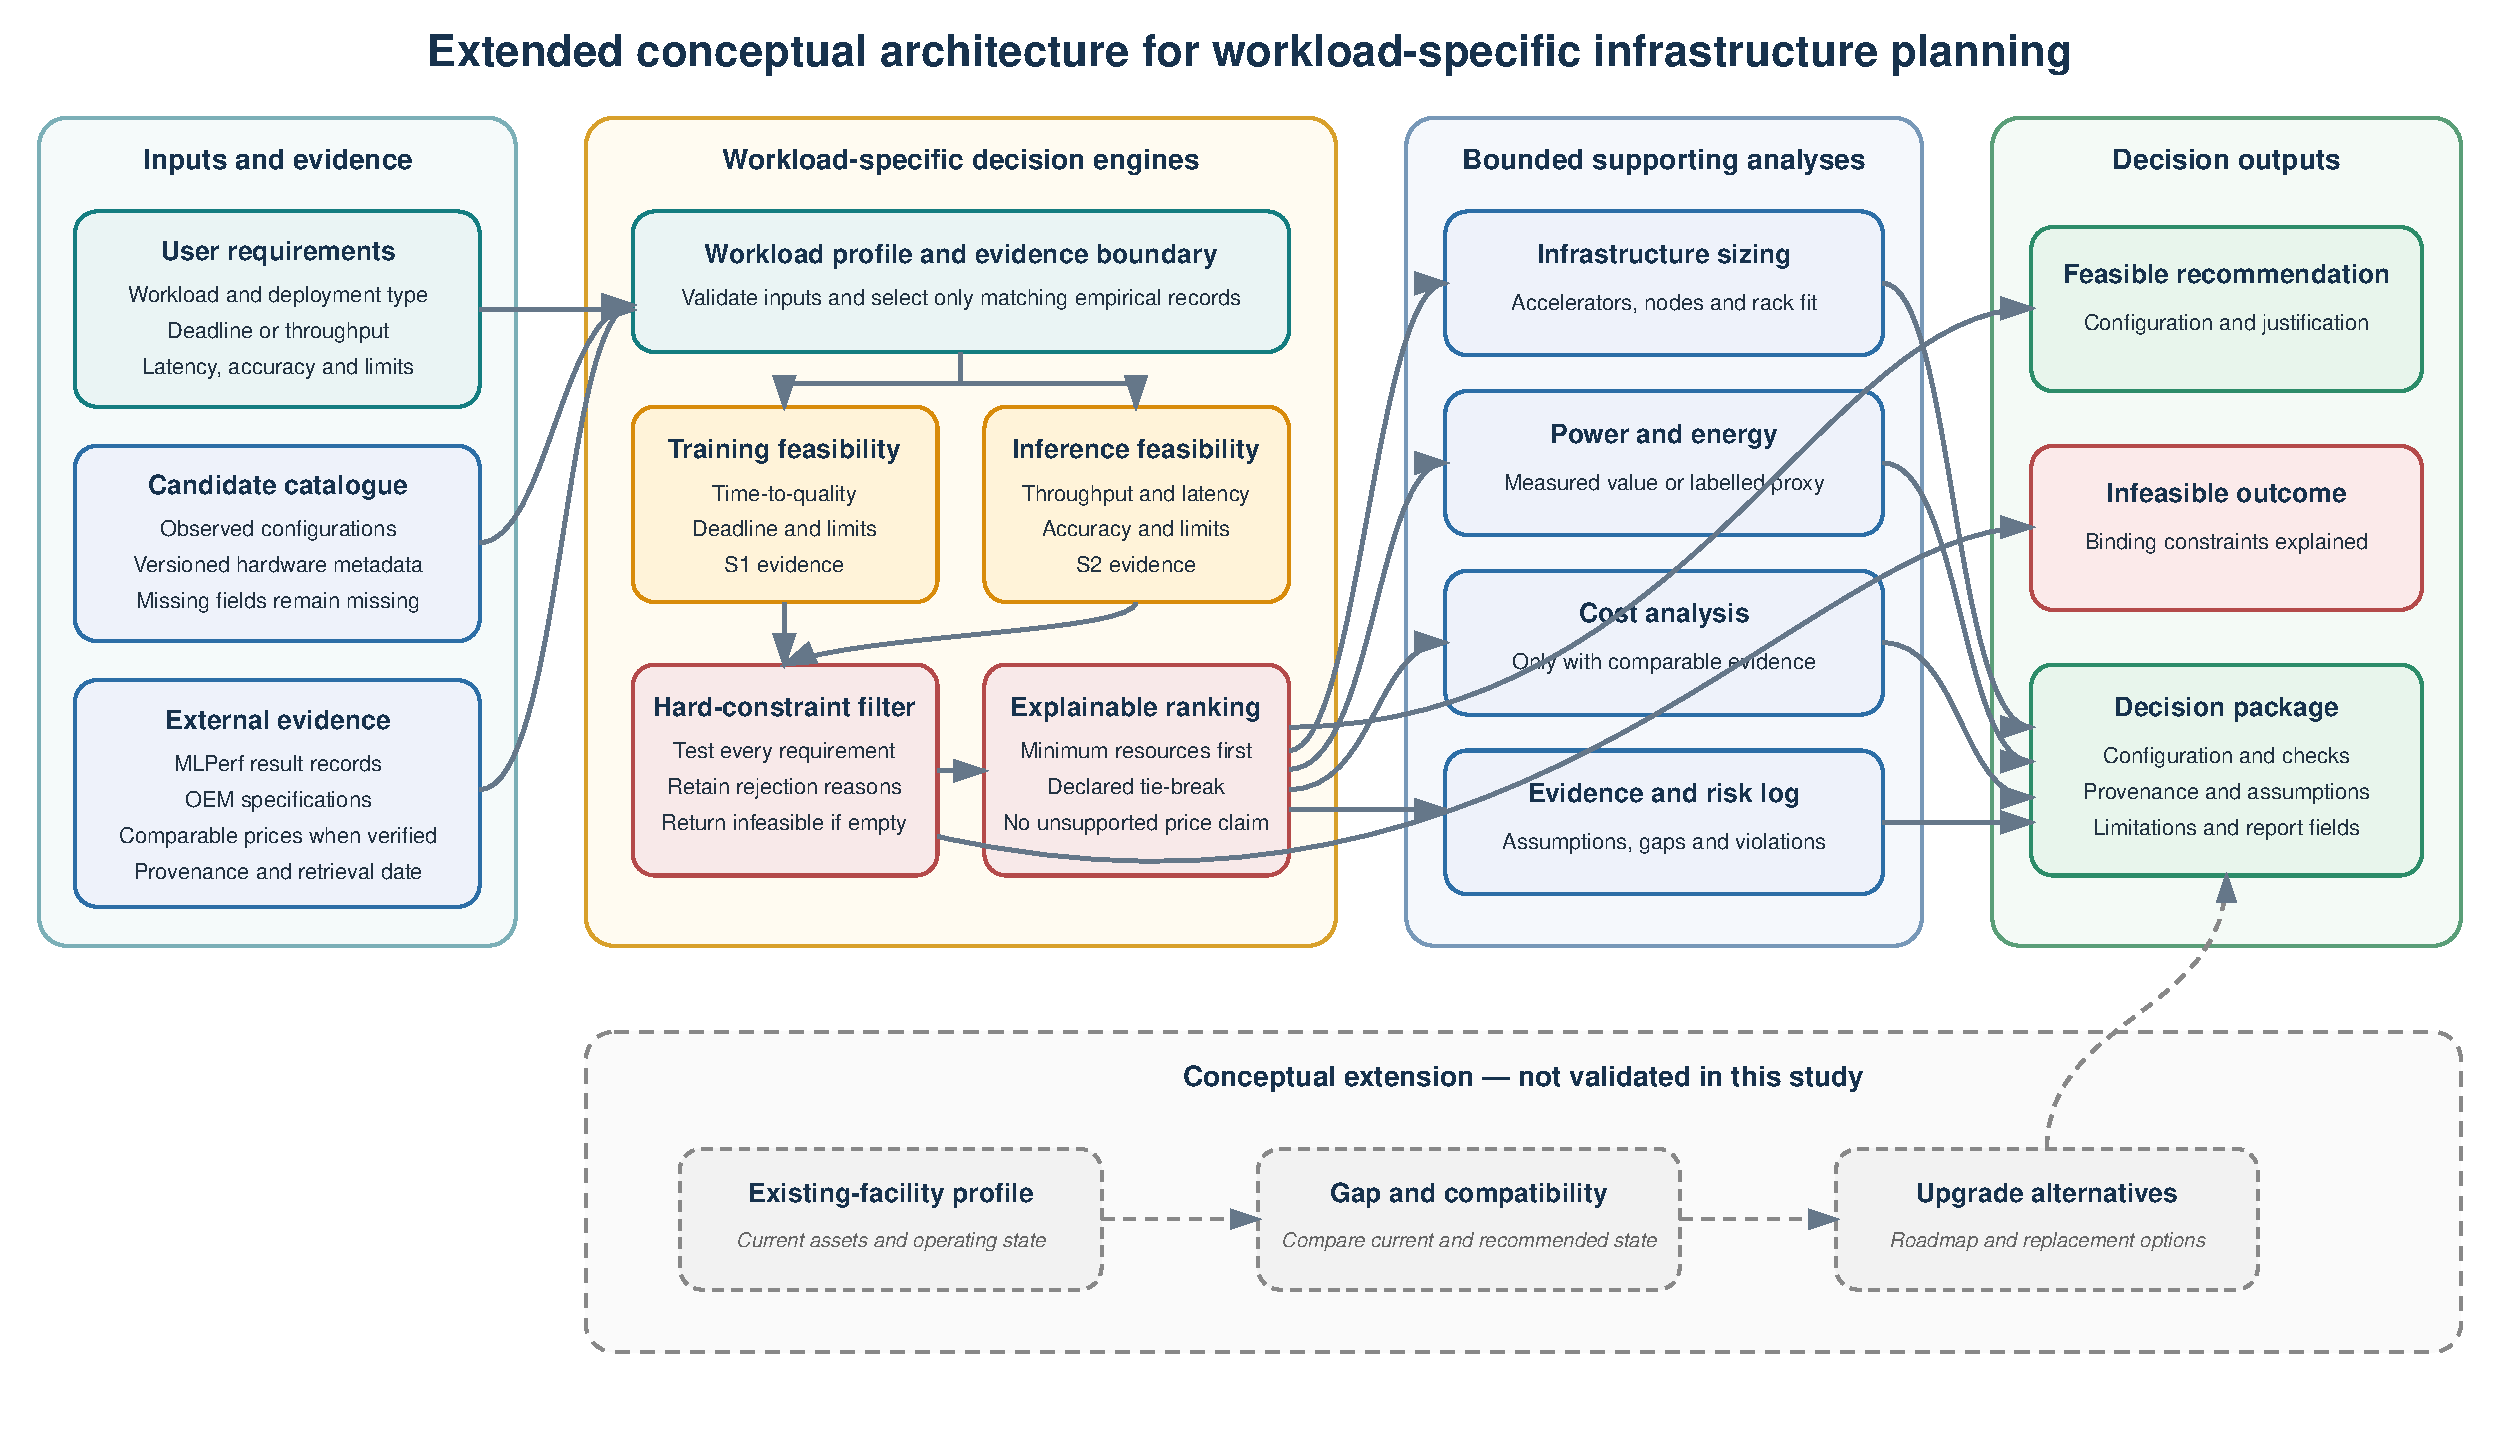
\includegraphics[width=0.96\textheight]{figures/extended_conceptual_architecture.pdf}
  \caption{Extended conceptual architecture for the wider infrastructure-planning prototype. The diagram records the intended end-to-end design while distinguishing future extensions with dashed borders and connectors. This paper validates only the workload-specific S1/S2 feasibility path and its bounded supporting checks; the existing-facility, complete cost and cooling, external-integration, and extended-reporting functions are not presented as implemented or experimentally validated.}
  \label{fig:conceptualarchitecture}
\end{sidewaysfigure}

\subsection{Decision Procedure and Explanation Record}


% Word blocks 66; 3.3 Decision Procedure and Explanation Record, paragraph 1
Both routines use an identical control flow. Whilst the actual calculations are very different, you can see how the process works from Table 2. We’ve written this without any form of language so you don’t get confused with any language semantics. Firstly, there is a screening process. Any hardware configurations which cross any strict boundaries will be excluded from being used. Every check will write a line of information to the audit log detailing what the empirical value was, what the target value was, whether it passed or failed and where the data originated from. This makes checking our sizing decisions easy to do. If there is a complete failure on validation, we still gain some debugging information. We have written the software to avoid any of these common shortcuts. Firstly, the code doesn’t take a runtime on a single GPU and extrapolate to work out scaling metrics for a large cluster. Secondly, if there isn’t data centre cost sheets or power information this isn’t just assumed to be zero. Lastly, we do not allow soft scoring to hide any failures on the infrastructure. All of these can be seen in the automated testing repo.


\begin{table}[htbp]
\caption{Common Decision Procedure}
\label{tab:procedure}
\centering
\footnotesize
\setlength{\tabcolsep}{3pt}
\renewcommand{\arraystretch}{1.08}
\begin{tabularx}{\columnwidth}{p{1.0cm}X}
\toprule
\textbf{Step} & \textbf{Operation}\\
\midrule
1 & Validate units, positive limits, and required fields.\\
2 & Select the workload-specific empirical catalogue.\\
3 & Evaluate every applicable hard constraint for every candidate.\\
4 & Store passing candidates in the feasible set and retain rejection reasons for all others.\\
5 & If the feasible set is empty, return \emph{infeasible} with the binding constraints.\\
6 & Otherwise apply the declared lexicographic ranking rule.\\
7 & Attach only those rack, power, energy, or cost outputs whose evidence requirements are satisfied.\\
8 & Export the decision, provenance, assumptions, and limitation flags.\\
\bottomrule
\end{tabularx}
\end{table}

\subsection{Training Feasibility Model}


% Word blocks 68; 3.4 Training Feasibility Model, paragraph 1
Let $\mathcal{C}_T$ be the set of observed training configurations. Candi-date $c$ has an observed time-to-quality $t_c$, accelerator count $g_c$, and optional engineering fields. For deadline $D$, and any declared resource, rack, or budget limits collected in $\boldsymbol{b}$, the feasible set is


\begin{equation}
\mathcal{F}_T(D,\boldsymbol{b})=\{c\in\mathcal{C}_T:t_c\leq D\ \wedge\ h_c(\boldsymbol{b})=1\},
\label{eq:trainset}
\end{equation}

% Word blocks 70; 3.4 Training Feasibility Model, paragraph 2
where $h_c$ = 1 means that every applicable non-performance constraint passes. If $\mathcal{F}_T$ is non-empty, the default recom-mendation is


\begin{equation}
c_T^*=\arg\min_{c\in\mathcal{F}_T}(g_c,t_c),
\label{eq:trainrank}
\end{equation}

% Word blocks 78; 3.4 Training Feasibility Model, paragraph 3
using lexicographic order: fewest accelerators first, then shorter observed time. This is a minimum-resource rule, not proof of minimum purchase price.


% Word blocks 79; 3.4 Training Feasibility Model, paragraph 4
For each submitted configuration, duration is calculated from the official start and stop timestamps. Following the benchmark aggregation represented in the source work-book, the largest and smallest of five durations are removed and the remaining three are averaged:


\begin{equation}
\bar t_c=\frac{1}{3}\sum_{i\in\mathcal{I}_c}t_{c,i}, \qquad
\mathcal{I}_c=\{1,\ldots,5\}\setminus\{\arg\min t,\arg\max t\}.
\label{eq:trimmed}
\end{equation}

% Word blocks 91; 3.4 Training Feasibility Model, paragraph 5
The raw-run audit remains independent of this arithmetic. It detected one log marked aborted in the Dell eight-GPU set; the record is retained and disclosed rather than silently deleted. Because it was also the maximum duration, it did not enter the three-run mean.


\subsection{Inference Feasibility Model}


% Word blocks 127,138; 3.5 Inference Feasibility Model, paragraph 1
Let candidate $c$ \ensuremath{\in} $\mathcal{C}_I$ have measured output-token through-put $q_c$, accelerator count $a_c$, p99 time to first token $f_c$, p99 time per output token $p_c$, and quality vector $\boldsymbol{r}_c$. For required throughput $Q$, maximum accelerators $A$, latency limits $F$ and $P$ , and quality thresholds $\boldsymbol{R}$,


\begin{multline}
\mathcal{F}_I=\{c\in\mathcal{C}_I:q_c\geq Q,\ a_c\leq A,\ f_c\leq F,\\
p_c\leq P,\ \boldsymbol{r}_c\succeq\boldsymbol{R},\ \text{result}_c=\mathrm{VALID}\}.
\label{eq:infset}
\end{multline}

% Word blocks 141; 3.5 Inference Feasibility Model, paragraph 2
The recommendation is


\begin{equation}
c_I^*=\arg\min_{c\in\mathcal{F}_I}(a_c,q_c-Q).
\label{eq:infrank}
\end{equation}

% Word blocks 144; 3.5 Inference Feasibility Model, paragraph 3
Thus the framework first minimizes accelerator count and then unused measured throughput. This deterministic tie-break explains why the eight-H100 system is preferred over the eight-H200 system at 20,000 and 30,000 output tokens/s. It does not assert that H100 is cheaper.


\subsection{Bounded Engineering Calculations}


% Word blocks 155; 3.6 Bounded Engineering Calculations, paragraph 1
S1 uses a rough operating-power estimate based on sourced records of 6.26 kW for a comparable eight-H100 ResNet training node \hyperref[ref:8]{[8]}. For a valid setup with proxy power $P_c$ (kW) and runtime $t_c$ (h),


\begin{equation}E_{\mathrm{IT},c}=P_ct_c,\end{equation}

\begin{equation}E_{\mathrm{facility},c}=\mathrm{PUE}\,E_{\mathrm{IT},c},\end{equation}

\begin{equation}H_c=3412.14P_c,\end{equation}

% Word blocks 159; 3.6 Bounded Engineering Calculations, paragraph 2
where energy is in kWh and $H_c$ is the computed heat rate in BTU/h. PUE was kept at 1.4 for the starting point and altered from1.2 and 1.6. The proxy was multiplied by node count for the two-node HPE and eight-node OCI setups. This is simple math for sensitivity analysis, not a direct telemetry of those submitted systems. Rack safety demands vendor maximum or inferred redundant protection instead of the operating-energy proxy. The distinction stops typical run power from being mistaken for an electrical design limit.


% Word blocks 160; 3.6 Bounded Engineering Calculations, paragraph 3
If a future deployment provides a separately verifiable and comparable accelerator-hour rate, the corresponding run cost can be computed as


\begin{equation}C_c=g_c\,t_c\,\rho,\end{equation}

% Word blocks 162; 3.6 Bounded Engineering Calculations, paragraph 4
where \ensuremath{\rho} is the correct accelerator-hour rate. The equation maps out a future cost extension; it is not evaluated numerically in this study because a dated, configuration-matched regional rate was not independently archived. On-premise capital-cost ranking is also omitted as comparable quotations were missing and hard to find.


\subsection{Reproducibility Design}


% Word blocks 165,166; 3.7 Reproducibility Design, paragraph 1
Each workflow has independent Python code base, machine-readable benchmark parameters, stated test cases, generated CSV or JSON outputs, and manual checks. The program skips assuming an untested configuration. Each disqualification records the failing condition. Validation combines: (i) source reconciliation; (ii) independent arithmetic for selected outputs; (iii) expected-result cases; (iv) deliberate invalid-input and hard-constraint tests; (v) workbook-to-Python comparison; and (vi) sensitivity sweeps. This method finds the transformation from evi-dence to decision, which is the real academic takeaway.


\section{Experimental Design}


\subsection{Data Acquisition, Extraction, and Reconciliation}


% Word blocks 170,171; 4.1 Data Acquisition, Extraction, and Reconciliation, paragraph 1
The measured figures were not pulled from a summary chart alone. For S1, the spec sheets and each raw result file were saved alongside their original MLCommons source links. Start time, stop time, final accuracy, global batch size, and run status were parsed into a tracked JSON sheet. The calculated runtime was recalculated from the timestamps Instead of typing it by hand. For S2, the performance summary, accuracy output, and system JSON for each chosen submission were Kept as distinct links in the benchmark CSV. The simulator processes these local, reviewable extracts; never relies on a live web request while running.


% Word blocks 172; 4.1 Data Acquisition, Extraction, and Reconciliation, paragraph 2
Three reconciliation layers cut down Data entry errors. First, the raw values are compared with the official result records. Second, a formula-based workbook separately tracks the same cases. Third, the Python output is compared with the expected workbook decision. The source record, workbook, and program therefore have distinct roles: source evidence provides the observations, the work-book makes the calculation visible to a reviewer, and Python establishes repeatable execution.


\begin{table}[htbp]
\caption{Evidence Used in the Two Experimental Scenarios}
\label{tab:evidence}
\centering
\footnotesize
\setlength{\tabcolsep}{3pt}
\renewcommand{\arraystretch}{1.1}
\begin{tabularx}{\textwidth}{p{2.2cm}XXXX}
\toprule
\textbf{Layer} & \textbf{S1 training} & \textbf{S2 inference} & \textbf{Permitted claim} & \textbf{Claim not permitted}\\
\midrule
Performance & 30 MLPerf v4.0 raw training logs & Four MLPerf v5.0 Server results & Feasibility among the observed configurations & Locally measured performance or untested scaling\\
Quality & Final ResNet-50 accuracy and run status & VALID flag and ROUGE-1/2/L thresholds & Benchmark quality condition passed & General model-quality superiority\\
System & Six MLPerf system disclosures & Four MLPerf system disclosures & Accelerator/node identity of each submission & Interchangeability of different software stacks\\
Physical & Matching Dell/HPE/OEM documents where available & Static accelerator/server metadata only & Bounded form-factor or conservative capacity check & Complete facility, cooling, or electrical design\\
Power & Comparable measured eight-H100 ResNet node & No matched operational record retained & S1 scenario proxy with explicit transfer limitation & Direct power comparison across submitted systems\\
Price & No independently archived comparable rate & No comparable price set & General cost-extension equation only & Any cheapest-system or numerical run-cost claim\\
\bottomrule
\end{tabularx}
\end{table}

\subsection{S1: ResNet-50 Training}


% Word blocks 176; 4.2 S1: ResNet-50 Training, paragraph 1
S1 relies on MLPerf Training v4.0 closed-division ResNet-50 v1.5 results on ImageNet with the 75.90\% quality target \hyperref[ref:10]{[10]}. Six H100 setups were chosen: Dell systems with four and eight GPUs, HPE Cray XD670 systems with eight and sixteen GPUs, and Oracle bare-metal configurations with eight and sixty-four GPUs. Five direct output files per configuration yielded 30 duration observations. Table 4 lists the derived representative times.


% Word blocks 177; 4.2 S1: ResNet-50 Training, paragraph 2
The core sensitivity parameter is the completion cutoff: 3, 5, 8, 10, 15, 20, 30, and 60 minutes. Additional con-trolled validations evaluate a two-minute infeasible deadline, rack-power rejection, PUE monotonicity, and explicit handling of cloud physical placement. No local ResNet-50 training was executed; acquiring the largest evaluated system would mandate 64 H100 accelerators.


\begin{table}[htbp]
\caption{S1 Evaluated Training Configurations}
\label{tab:s1configs}
\centering
\footnotesize
\setlength{\tabcolsep}{3pt}
\renewcommand{\arraystretch}{1.08}
\begin{adjustbox}{max width=\linewidth}
\begin{tabular}{lrrr}
\toprule
\textbf{ID} & \textbf{GPUs} & \textbf{Nodes} & \textbf{Time (min)}\\
\midrule
Dell-4G & 4 & 1 & 26.882\\
Dell-8G & 8 & 1 & 13.163\\
HPE-8G & 8 & 1 & 13.619\\
HPE-16G & 16 & 2 & 7.930\\
OCI-8G & 8 & 1 & 13.273\\
OCI-64G & 64 & 8 & 2.483\\
\bottomrule
\end{tabular}
\end{adjustbox}
\end{table}

% Word blocks 178; 4.2 S1: ResNet-50 Training, paragraph 3
The raw-run review also records dispersion before the trimmed aggregation. Table 5 details the coefficient of vari-ation (CV) across the five retrieved durations. Five setuos have CV below 0.16\%, proving very consistent iterated times. Dell-8G is the exception at 2.64\% because its fifth record is labeled aborted and has a duration of 13.944 minutes, compared with approximately 13.15–13.17 minutes for the four successful records. Disclosing this dif-ference matters: the final representative time is consistent after the predefined trimming rule, but the raw evidence is not described as five equivalent successful runs.


\begin{table}[htbp]
\caption{S1 Raw-Run Status and Dispersion}
\label{tab:s1quality}
\centering
\footnotesize
\setlength{\tabcolsep}{3pt}
\renewcommand{\arraystretch}{1.08}
\begin{adjustbox}{max width=\linewidth}
\begin{tabular}{lrrr}
\toprule
\textbf{ID} & \textbf{Successful} & \textbf{Aborted} & \textbf{CV (\%)}\\
\midrule
Dell-4G & 5 & 0 & 0.052\\
Dell-8G & 4 & 1 & 2.637\\
HPE-8G & 5 & 0 & 0.085\\
HPE-16G & 5 & 0 & 0.158\\
OCI-8G & 5 & 0 & 0.050\\
OCI-64G & 5 & 0 & 0.043\\
\bottomrule
\end{tabular}
\end{adjustbox}
\end{table}

\subsection{S2: Llama 2 70B Online Inference}


% Word blocks 182; 4.3 S2: Llama 2 70B Online Inference, paragraph 1
S2 relies on four HPE closed-division MLPerf Inference v5.0 results for Llama 2 70B, the OpenOrca dataset, Server scenario, and the 99\%-of-FP16 accuracy target \hyperref[ref:11]{[11]}. Table 6 evaluates the fields imported into the simulation. Every row was marked VALID and passed the published TTFT, TPOT, and ROUGE thresholds. The study uses the p99 latency limits recorded with these results: 2.0 s for TTFT and 0.2 s for TPOT.


% Word blocks 183,184; 4.3 S2: Llama 2 70B Online Inference, paragraph 2
Six prescribed workload profiles vary throughput and maximum accelerator count. The throughput contraints are 4,000, 8,000, 20,000, 20,000, 30,000, and 32,000 output tokens/s; the corresponding accelerator ceilings are 1, 2, 2, 8, 8, and 8. A 99-case matrix then varies throughput and resource limits to evaluate decision boundaries. S2 does not calculate power or financial cost because equivalent operational power and comparable purchase-price evidence were missing.


\begin{table}[htbp]
\caption{S2 Official MLPerf Inference v5.0 Inputs}
\label{tab:s2configs}
\centering
\footnotesize
\setlength{\tabcolsep}{3pt}
\renewcommand{\arraystretch}{1.08}
\begin{adjustbox}{max width=\linewidth}
\begin{tabular}{lrrrrrr}
\toprule
\textbf{Configuration} & \textbf{Accelerators} & \textbf{Output tok/s} & \textbf{p99 TTFT (s)} & \textbf{p99 TPOT (s)} & \textbf{ROUGE-1} & \textbf{Result}\\
\midrule
HPE-GH200-1 & 1 & 4,327.68 & 1.8895 & 0.1909 & 44.5531 & VALID\\
HPE-GH200-2 & 2 & 8,674.58 & 0.8064 & 0.1712 & 44.5503 & VALID\\
HPE-H100-8 & 8 & 30,498.87 & 1.2950 & 0.1429 & 44.4303 & VALID\\
HPE-H200-8 & 8 & 31,281.09 & 0.6660 & 0.1685 & 44.5663 & VALID\\
\bottomrule
\end{tabular}
\end{adjustbox}
\end{table}

\section{Results}


\subsection{S1 Training Feasibility}


% Word blocks 239,262; 5.1 S1 Training Feasibility, paragraph 1
Figure 4 depicts the profiled training times. Increasing scale reduced time-to-quality threshold, but the  allocation was dictated by the latency bound rather than by speed alone. The 30- and 60-minute scenarios nominated Dell-4G. The 15- and 20-minute runs selected Dell-8G. The 8- and 10-minute instances mandated HPE-16G, and the 3- and 5-minute cases mandated OCI-64G. A two-minute deadline proved unattainable. These shifts answer RQ1 and RQ2 for training workloads: the same workload binds to different resources when the service requirement changes. Figure 3 renders these decision limits visible. A dead-line underneath an observed execution time alters the feasible set discontinuously; the selection is there-fore a step function rather than a smooth hardware-sizing curve. This behavior is intentional. Between observed coordinates, the framework does not fabricate a fractional accelerator requirement or estimate a new system. Table 7 details the complete feasibility matrix grid. A verification indicates that the tracked time duration is within the contraint; the selected row is the feasible configuration with the fewest GPUs and then the shorter time.


\begin{figure}[htbp]
  \centering
  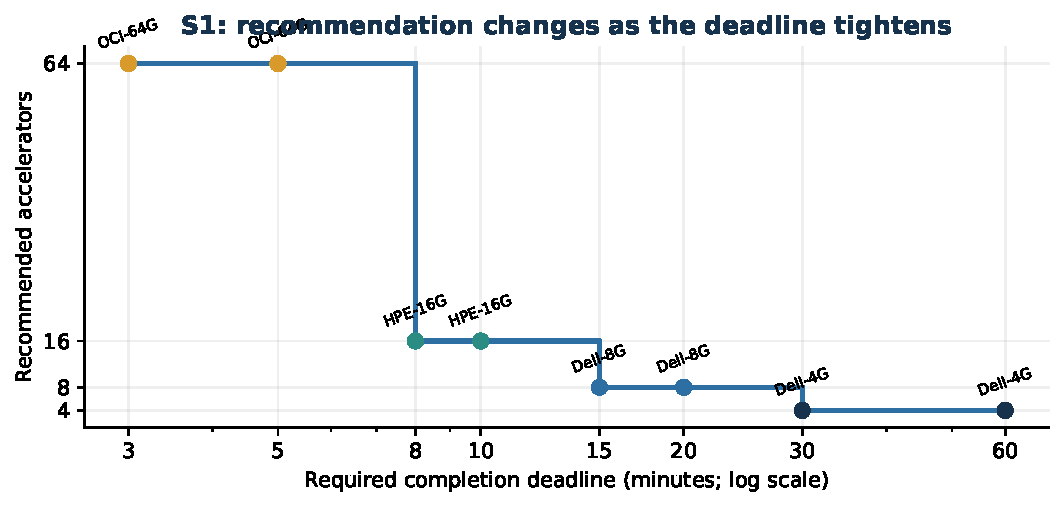
\includegraphics[width=\columnwidth]{s1_deadline_map.pdf}
  \caption{S1 deadline sensitivity. The recommendation changes only when another observed configuration becomes necessary.}
  \label{fig:s1deadline}
\end{figure}

\begin{table}[htbp]
\caption{S1 Deadline Feasibility Matrix}
\label{tab:s1deadline}
\centering
\footnotesize
\setlength{\tabcolsep}{3pt}
\renewcommand{\arraystretch}{1.08}
\begin{adjustbox}{max width=\linewidth}
\begin{tabular}{rrrrrrrrl}
\toprule
\textbf{Deadline} & \textbf{Dell-4G} & \textbf{Dell-8G} & \textbf{HPE-8G} & \textbf{HPE-16G} & \textbf{OCI-8G} & \textbf{OCI-64G} & \textbf{Min. GPUs} & \textbf{Recommendation}\\
\midrule
3 min  & -- & -- & -- & -- & -- & Pass & 64 & OCI-64G\\
5 min  & -- & -- & -- & -- & -- & Pass & 64 & OCI-64G\\
8 min  & -- & -- & -- & Pass & -- & Pass & 16 & HPE-16G\\
10 min & -- & -- & -- & Pass & -- & Pass & 16 & HPE-16G\\
15 min & -- & Pass & Pass & Pass & Pass & Pass & 8 & Dell-8G\\
20 min & -- & Pass & Pass & Pass & Pass & Pass & 8 & Dell-8G\\
30 min & Pass & Pass & Pass & Pass & Pass & Pass & 4 & Dell-4G\\
60 min & Pass & Pass & Pass & Pass & Pass & Pass & 4 & Dell-4G\\
\bottomrule
\end{tabular}
\end{adjustbox}
\end{table}

% Word blocks 263; 5.1 S1 Training Feasibility, paragraph 2
Within the eight-GPU cluster, Dell-8G, HPE-8G, and OCI-8G finished within 13.163, 13.619, and 13.273 minutes, respec-tively. These are indicative cross-system observations, not controlled vendor rankings, because the submitted stacks differ. Within-family comparisons are more interpretable: moving HPE from 8 to 16 GPUs minimized time from 13.619 to 7.930 minutes (a 41.8\% lowered, rather than an optimal 50\%), while moving OCI from 8 to 64 GPUs reduced time from 13.273 to 2.483 minutes (an 81.3\% reduction, rather than the 87.5\% optimal under strict eightfold scaling). The findings warns against using accelerator count as a linear performance predictor.


\begin{figure}[htbp]
  \centering
  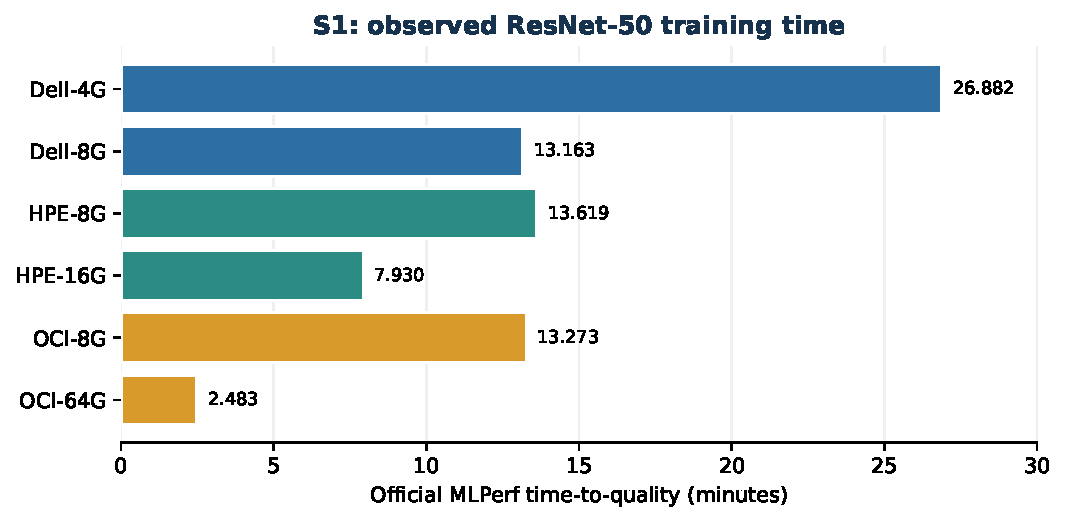
\includegraphics[width=\columnwidth]{s1_training_time.pdf}
  \caption{S1 representative time-to-quality derived from official MLPerf Training v4.0 raw timestamps. Lower is better.}
  \label{fig:s1time}
\end{figure}

% Word blocks 264,265; 5.1 S1 Training Feasibility, paragraph 3
The base power surrogate generates facility-energy estimates of 1.923 kWh/run for Dell-8G, 1.989 for HPE-8G, 2.317 for HPE-16G, 1.939 for OCI-8G, and 2.902 for OCI-64G at PUE 1.4. Dell-4G is purposefully excluded since no equivalent four-GPU node power value was archived. The fastest option therefore did not have the lowest proxy energy per com-pleted run. This is a qualified comparison under a common cross-study calibration, not measured facility energy.


% Word blocks 266,302; 5.1 S1 Training Feasibility, paragraph 4
Table 8 illustrates the PUE sensitivity visibly. Shifting from PUE 1.2 to 1.6 increases every facility calculation by one third because workload execution window and IT surrogate power remain persistent. This is a valid internal coherance test, but it is not evidence that any profiled site actually performs at one of these PUE values. Annual figures in the workbook spreadhseet assume one equivalent completed run per day; the paper highlights per-run values because the annual frequency is a case-study assumption rather than an recorded operating timeline.


\begin{table}[htbp]
\caption{S1 Facility-Energy Proxy Under PUE Sensitivity (kWh/run)}
\label{tab:pue}
\centering
\footnotesize
\setlength{\tabcolsep}{3pt}
\renewcommand{\arraystretch}{1.08}
\begin{adjustbox}{max width=\linewidth}
\begin{tabular}{lrrr}
\toprule
\textbf{ID} & \textbf{PUE 1.2} & \textbf{PUE 1.4} & \textbf{PUE 1.6}\\
\midrule
Dell-8G & 1.648 & 1.923 & 2.197\\
HPE-8G & 1.705 & 1.989 & 2.274\\
HPE-16G & 1.986 & 2.317 & 2.648\\
OCI-8G & 1.662 & 1.939 & 2.216\\
OCI-64G & 2.487 & 2.902 & 3.316\\
\bottomrule
\end{tabular}
\end{adjustbox}
\end{table}

% Word blocks 303,289; 5.1 S1 Training Feasibility, paragraph 5
The rack sensitivity employs a different validation class. Dell-8G uses an 11.5-kW provisioning cap; HPE-8G and HPE-16G use 12 and 24 kW calculated net capacities. All three populate one assumed rack at 40, 80, and 120 kW bounds when space and weight also qualify. A knowingly 10-kW test drops the Dell node. The outcome showcases constraint behavior, not vendor validation of a particular rack deployment.


% Word blocks 290; 5.1 S1 Training Feasibility, paragraph 6
No quantitative cloud-cost comparison is documented because the exact regional price, service identifier, currency, and retrieval log could not be independently logged to the same evidence standard as the benchmark results. The framework hence reports technical feasibility and minimum-resource ranking only. It does not conclude which cloud or local system has the lowest monetary cost.


\subsection{S2 Inference Feasibility}


% Word blocks 304; 5.2 S2 Inference Feasibility, paragraph 1
Figure 5 illustrates the four profiled throughput coordinates and the 20,000-token/s example threshold. Table 9 details the specified results. The one and two-GH200 configurations matched the 4,000- and 8,000-token/s scenarios. Neither could satisfy 20,000 tokens/s under a two-accelerator bound, so T3 accurately returned unattaunable. Modifying the ceiling to eight apermitted both H100-8 and H200-8 to pass. Equaion (5) nominated H100-8 because both use eight accelerators and H100-8 has the smaller surplus above the bound. The same rule selected H100-8 at 30,000 tokens/s. At 32,000 tokens/s, even H200-8 shortfalled by 718.91 tokens/s, producing another justified infeasible outcome.


\begin{figure}[htbp]
  \centering
  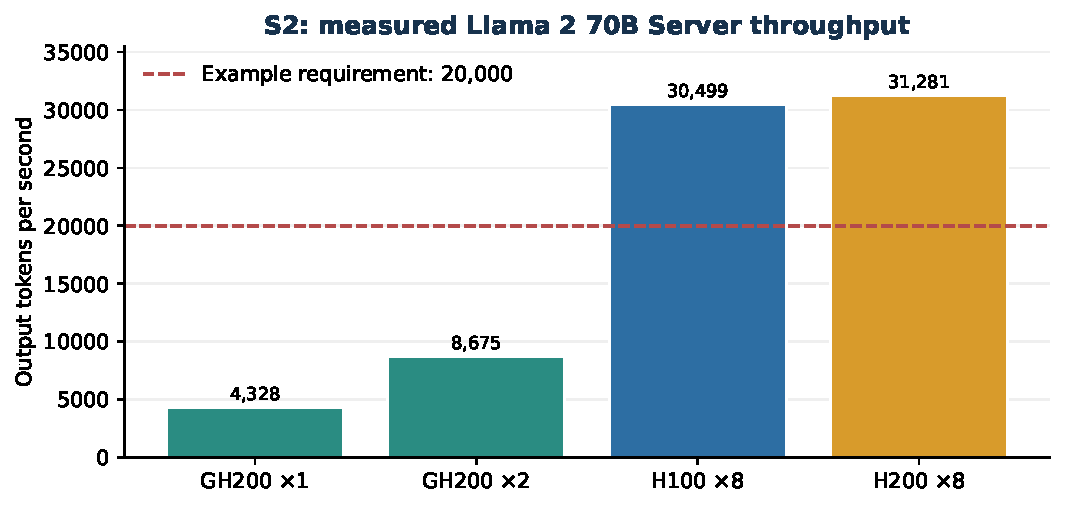
\includegraphics[width=\columnwidth]{s2_throughput.pdf}
  \caption{S2 measured output-token throughput. The dashed line illustrates T4’s 20,000-token/s requirement; latency and accuracy must also pass.}
  \label{fig:s2throughput}
\end{figure}

% Word blocks 305; 5.2 S2 Inference Feasibility, paragraph 2
Throughput exclusively did not determine feasibility. All four baseline records already met the 2.0-s TTFT bound, 0.2-s TPOT limit, validity flag, and quality thresholds. Separate tests restricted each condition until no candidate passed, verifying that the implementation treats them as hard constraints. The result resolves RQ1: the shared architecture can support inference, but only through a requirement vector different from training’s deadline rule.


\begin{table}[htbp]
\caption{S2 Predefined Cases and Python Decisions}
\label{tab:s2cases}
\centering
\footnotesize
\setlength{\tabcolsep}{3pt}
\renewcommand{\arraystretch}{1.08}
\begin{adjustbox}{max width=\linewidth}
\begin{tabular}{crrl}
\toprule
\textbf{Case} & \textbf{Tok/s} & \textbf{Max acc.} & \textbf{Decision}\\
\midrule
T1 & 4,000 & 1 & GH200-1\\
T2 & 8,000 & 2 & GH200-2\\
T3 & 20,000 & 2 & Infeasible\\
T4 & 20,000 & 8 & H100-8\\
T5 & 30,000 & 8 & H100-8\\
T6 & 32,000 & 8 & Infeasible\\
\bottomrule
\end{tabular}
\end{adjustbox}
\end{table}

% Word blocks 306,351; 5.2 S2 Inference Feasibility, paragraph 3
The 99-case sensitivity grid gives a vast view than the six isolated examples. Figure 6 varies the target rate from 2,000 to 34,000 output tokens/s and the accelerator ceiling across one, two, and eight devices. With single accelerator, feasibility terminates after the 4,000-token/s point because GH200-1 registers 4,327.68. With two accelerators, GH200-2 remains available through 8,000 tokens/s. Under the eight-accelerator ceiling, H100-8 becomes the preferred observed system from 9,000 through 30,000 tokens/s. At 31,000 to-kens/s, H100-8 is insufficient and H200-8 is selected. From 32,000 tokens/s onward, the observed catalogue is infeasi-ble. These transitions follow the measurements exactly; they are not rounded capacity forecasts.


\begin{figure}[htbp]
  \centering
  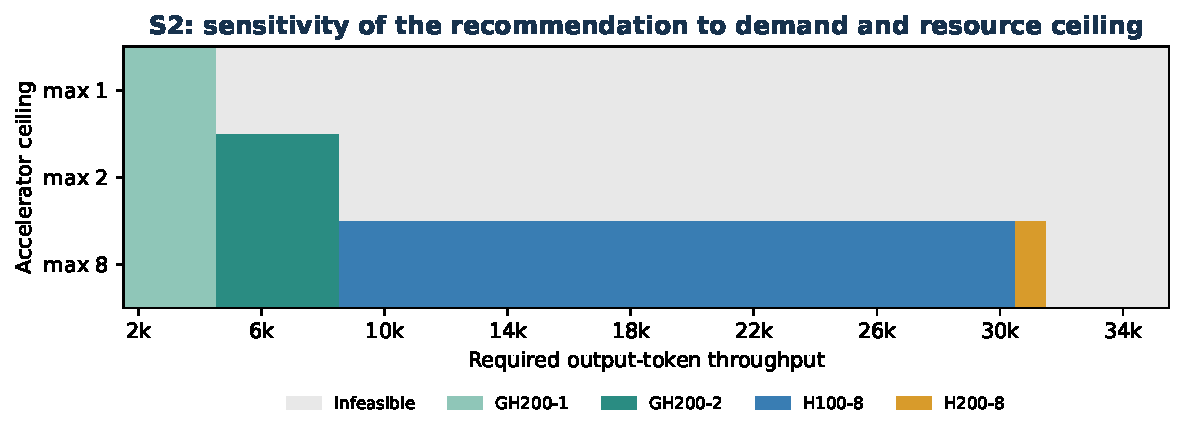
\includegraphics[width=0.92\textwidth]{s2_sensitivity_map.pdf}
  \caption{S2 sensitivity across 99 combinations of throughput requirement and accelerator ceiling. Grey cells are infeasible among the four observed candidates.}
  \label{fig:s2sensitivity}
\end{figure}

% Word blocks 352; 5.2 S2 Inference Feasibility, paragraph 4
Table 10 itemizes the explanation record for T4. GH200-1 and GH200-2 fail throughput even though they clear the accelerator ceiling and baseline quality/latency parameters. Both eight-accelerator systems pass. H100-8 is isolated only after filtering, through the minimum-surplus tie-break. This logging distinguishes a disqualification basis from a ranking factor.


\begin{table}[htbp]
\caption{Illustrative Candidate-Level Explanation for T4 (20,000 Output Tokens/s, Maximum Eight Accelerators)}
\label{tab:t4explanation}
\centering
\footnotesize
\setlength{\tabcolsep}{3pt}
\renewcommand{\arraystretch}{1.08}
\begin{tabularx}{\textwidth}{p{1.8cm}p{2.2cm}p{1.9cm}p{1.2cm}p{1.2cm}p{1.3cm}X}
\toprule
\textbf{Candidate} & \textbf{Throughput} & \textbf{Acc. limit} & \textbf{TTFT} & \textbf{TPOT} & \textbf{Quality} & \textbf{Outcome and reason}\\
\midrule
GH200-1 & Fail & Pass & Pass & Pass & Pass & Rejected: observed throughput below 20,000\\
GH200-2 & Fail & Pass & Pass & Pass & Pass & Rejected: observed throughput below 20,000\\
H100-8 & Pass & Pass & Pass & Pass & Pass & Feasible and selected: eight accelerators, smaller surplus\\
H200-8 & Pass & Pass & Pass & Pass & Pass & Feasible but not selected: equal count, larger surplus\\
\bottomrule
\end{tabularx}
\end{table}

\subsection{Validation Summary}


% Word blocks 355; 5.3 Validation Summary, paragraph 1
Table 11 condenses the replicability proof. Six data backed S1 tests were retained after the three cost sensitive cases were omitted. S2 cleared eighteen unit tests, replicated all six workbook cases, and produced 99 sensitivity records. Manual audits reproduced the Dell-8G energy arithmetic and extracted S2 throughput-per-accelerator and latency-buffer values. Invalid non-positive parameters were dropped. Tests also verified that cloud rack placement remains “provider managed,” missing prices are not assumed, and S2 does not label its recommendationlowest cost.


% Word blocks 356; 5.3 Validation Summary, paragraph 2
The evaluation proves exact agreement be-tween source records, formulas, Python, and workbook cases. It does not separately verify the physical metrics disclosed by MLCommons. That distinction addresses RQ3: the evidence supports the framework’s transformation and boundary handling, while the benchmark organization remains the source of the underlying performance measurements.


% Word blocks 339,357; 5.3 Validation Summary, paragraph 3
The checks span exceed predicted recommendations. S1 evaluates an impossible deadline, a single-candidate boundary, a rack-power rejection, visibility of an aborted log, mono-tonic PUE behavior, and cloud rack semantics. S2 checks record counts and exact throughput reconciliation; all six expected cases; the effect of relaxing an accelerator ceiling; deterministic tie handling; the narrow interval in which H200-8 is selected; requirements above the observed maximum; independent TTFT, TPOT, and accuracy rejections; manual arithmetic; the explicit absence of price optimization; and invalid non-positive input handling. The entire Catalogue is detailed in Appendix A.


% Word blocks 358; 5.3 Validation Summary, paragraph 4
Sensitivity and unit testing resolve distinct questions. The unit cases ask whether a defined threshold triggers the expected output. The sensitivity grid asks whether decisions remain coherent over a wider input space. Nei-ther dynamic demonstrates completeness of the candidate catalogue, but combined they mitigate the six headline cases merely reflect manual interpretation.


\begin{table}[htbp]
\caption{Reproducibility and Validation Evidence}
\label{tab:validation}
\centering
\footnotesize
\setlength{\tabcolsep}{3pt}
\renewcommand{\arraystretch}{1.08}
\begin{tabularx}{\columnwidth}{Xrr}
\toprule
\textbf{Check} & \textbf{S1} & \textbf{S2}\\
\midrule
Official evaluated configurations & 6 & 4\\
Raw performance logs/records & 30 & 4\\
Predefined result cases & 8 deadlines & 6 cases\\
Automated checks retained and passed & 6/6 & 18/18\\
Workbook cases reproduced & Yes & 6/6\\
Sensitivity cases & PUE/rack & 99\\
Local model execution & No & No\\
\bottomrule
\end{tabularx}
\end{table}

\section{Discussion}


\subsection{What the Two Scenarios Establish}


% Word blocks 362; 6.1 What the Two Scenarios Establish, paragraph 1
The unified outcome is more pragmatic than a single “optimal GPU” statement. In S1, the core performance variable is elapsed time to a defined quality target. Conversely, inside S2, the core metrics are output-token rate, tail latency, and accuracy under a Server workload. The framework architecture can be unifoed, but the feasibility predicate cannot. A generic accelerator-count formula would obscure this difference and invite unsubstantiated extrapolation.


% Word blocks 363; 6.1 What the Two Scenarios Establish, paragraph 2
The experiments further demonstrate why infeasibility is a valid planning outcome. T3 does not fail because the accelerator type is structurally incompatible; it fails because none of the recorded one- or two-accelerator systems reaches 20,000 output tokens/s. T6 fails for a different reason: the demand is above the fastest observed candidate even when eight accelerators are allocated. Reporting the failed conditions is more defensible than proposing an untested configuration.


% Word blocks 364; 6.1 What the Two Scenarios Establish, paragraph 3
Ranking must remain segregated from filtering. An option that fails a single strict condition cannot fix it by doing well on another. Not until all conditions clears does the standard rule lower accelerator count. The backup tie-break cuts out waste, which avoids showing unnecessary measured capacity as beneficial by default. Different organizations can switch the tie-break with power, budget, vendor policy, or risk once similar proof exists; the hard-constraint layer would remain exactly as it is.


\subsection{Power and Cost Interpretation}


% Word blocks 366; 6.2 Power and Cost Interpretation, paragraph 1
S1 shows an critical evidence discipline. The 6.26-kW figure is taken from a comparable tracked test, rather than the chosen Dell, HPE, or Oracle MLPerf systems. Scaling it by nodes makes it easy to calculate an internally consistent stress test, but cannot reveal actual whole-system energy. Just like that, PUE converts IT power into a facility estimate; It isn't a real reading of the cooling plant. For electrical safety, vendor maximum or PSU-capacity evidence is the relevant conservative input. These quantities should never be collapsed into one column labelled simply “power.”


% Word blocks 402; 6.2 Power and Cost Interpretation, paragraph 2
Cost claims require the same validation. No numerical cloud comparison is included because the exact regional price record was not independently logged. Dell/HPE acquisition cost also depends on a complete configuration, support, region, taxes, and quotation date. In the absence of verified data, minimum-resource technically feasible is the correct label. Any claim that the framework identifies the  most economical cloud or on-premise system would be baseless.


\subsection{Relationship to the Prototype Catalogue}


% Word blocks 404; 6.3 Relationship to the Prototype Catalogue, paragraph 1
The catalogue documentation and experiments serve dif-ferent purposes. The catalogue is an implementation deliverables: after normalization and provenance review, it can hydrate filters for form factor, memory, electrical characteristics, networking, storage, racks, PDUs, and related equipment. S1 and S2 are research proof: they validate expected decisions for precisely defined workloads and can become validation gates for the future prototype.


% Word blocks 392,394,405; 6.3 Relationship to the Prototype Catalogue, paragraph 2
decoupling the layers mitigates two errors. First, the exixtance of a product row does not mean its workload performance has been quantified. Second, a benchmark sub-mission does not provide every attribute needed for facility engineering. A production implementation should use concsiatent entity identifiers, normalize the vertically concatenated storage and networking tables, remove duplicate datasets, differentiate manufacturer facts from estimates, and attach field-level lineage and retrieval dates. The current paper does not claim that this data-engineering work has been finalzed.


\subsection{Threats to Validity and Limitations}


% Word blocks 408; 6.4 Threats to Validity and Limitations, paragraph 1
The study has five primary constraints. First, it is a post-hoc, trace-driven assessment. ResNet-50 was not re-trained and Llama 2 70B inference was not run on local hardware. The study hence cannot empirically identify measurement error in the official results. Second, broader applicability is restricited by the chosen benchmark versions, models, datasets, precision/quality targets, systems, and software stacks. A different model or serving strategy may change the sequence.


% Word blocks 409,411; 6.4 Threats to Validity and Limitations, paragraph 2
Third, the candidate space is limited. The framework choses among recorded configurations; it does not forecast arbitary counts or merge components into an uevaluated system. This contraint reduces scope but preserves the credibility of the recommendation. Fourth, S1’s energy values are early stage estimations and S2 has no operational-energy output. Comprehensive monitoring under synchronized conditions would be required for a comparative energy claim. Fifth, exact on-premise price optimization is unaddressed. Matched dated vendor bids are needed before a financial grading can be justified.


% Word blocks 412; 6.4 Threats to Validity and Limitations, paragraph 3
The experiment also uses benchmarking constants rather than requirements gathered from an operating organization. Deadlines, accelerator bounds, PUE, rack limits, and bud-gets therefore illustrate decision patterns, not standard scoping defaults. Regardless, the cases are reppricable, include extremes, and disclose rather than mask the assumptions on which the results lean.


\subsection{Next Implementation and Research Steps}


% Word blocks 415; 6.5 Next Implementation and Research Steps, paragraph 1
The upcoming operational task is to adapt the documented catalogue into a normalized, versioned schema and present the two simulation engines through one inter-face. The six S2 profiles, S1 deadline sweep, and regulated tests should be maintained as regression tests. A configuration should enter the performance catalogue only when its benchmark profile and provenance are finalized.


% Word blocks 416; 6.5 Next Implementation and Research Steps, paragraph 2
Extended research should add synchronized whole-system power metrics, replicable on-premise proposals, and extra workloads without changing theverification criteria. Only after those inputs are available should the framework streamline operational energy or total financial cost. A physical verification study could run smaller accessible models locally and cross reference recorded metrics with framework decisions. In-depth cooling, electrical backup, structural loading, and site design should remain subject to competent engineering scrutiny rather than being deduced from the current simulation.


\section{Conclusion}


% Word blocks 420; 7 Conclusion, paragraph 1
This paper proposed WISP-DC, a workload-aware viability framework validated with official MLPerf traces and reproducible Python simulations. The training scenario demostrated that the minimum-accelerator recommendation for the same ResNet-50 workload moved from 4 to 8, 16, and 64 H100 GPUs as the deadline compresses; a two-minute target was unattainable among the six profiled configurations. The inference scenario showed that Llama 2 70B demands must be analyzed collectively: 20,000 output tokens/s was in-feasible with at most two accelerators but feasible with eight, while 32,000 tokens/s was outside all four observed systems. The maintained data-backed realizations passed 24 automated audits in total, and S2 replicated all six predefined cases across an additional 99-case sensitivity grid.


% Word blocks 421; 7 Conclusion, paragraph 2
The core finding is knowingly focused. Official benchmark proof can validate an verifiable early feasibility decision when each workload uses its own execution semantics, hard limits are applied before ranking, and omitted evidence is not replaced by an assumption. The paper verifies that decision process. It does not assert new model-performance measurements, full facility engineering, logged S2 energy, or the lowest cost on-premise purchase. Those boundaries make the current result useful as a defen-sible research baseline and a set of acceptance tests for the intended prototype.


\appendix
% Preserve the original paper's table, figure and equation numbering.
\counterwithout{equation}{section}
\setcounter{equation}{9}
\renewcommand{\theequation}{\arabic{equation}}
\renewcommand{\thetable}{\arabic{table}}
\renewcommand{\thefigure}{\arabic{figure}}

\section{Complete Validation Inventory}


% Word blocks 424; Appendix A Complete Validation Inventory, paragraph 1
Tables 12 and 13 tabulate the performed audits maintained in the produced validation outputs. They are incorporated to make the meaning of “validated simulation” concrete. A pass indicates that the current code generated the slated targeted behavior; it does not mean that the test empirically repeated an MLPerf workload.


\begin{table}[htbp]
\caption{S1 Controlled Validation Checks}
\centering
\footnotesize
\setlength{\tabcolsep}{3pt}
\renewcommand{\arraystretch}{1.12}
\begin{tabularx}{\textwidth}{p{0.9cm}X X p{1.2cm}}
\toprule
\textbf{ID} & \textbf{Test input or condition} & \textbf{Expected behavior} & \textbf{Result}\\
\midrule
CT-01 & Two-minute training deadline & No evaluated configuration is fea-sible & Pass\\
CT-02 & Three-minute training deadline & OCI-64G is the only feasible config-uration & Pass\\
CT-03 & 10-kW rack limit applied to 11.5-kW Dell planning maxi-mum & Candidate is rejected by rack-power constraint & Pass\\
CT-04 & Audit all raw Dell-8G statuses & Exactly one aborted log is exposed & Pass\\
CT-05 & Increase PUE from 1.2 to 1.4 to 1.6 & Facility-energy estimate increases strictly & Pass\\
CT-06 & Request physical rack output for OCI & Outputremainsprovider-managed; no rack is fabricated & Pass\\
\bottomrule
\end{tabularx}
\end{table}


\begin{table}[htbp]
\caption{S2 Automated Validation Checks}
\centering
\footnotesize
\setlength{\tabcolsep}{3pt}
\renewcommand{\arraystretch}{1.12}
\begin{tabularx}{\textwidth}{p{0.65cm}X X p{1.2cm}}
\toprule
\textbf{No.} & \textbf{Check} & \textbf{Purpose} & \textbf{Result}\\
\midrule
1 & Four official configurations load & Detect missing or duplicated catalogue records & Pass\\
2 & Throughput values equal retained offi-cial extracts & Detect transcription or parsing error & Pass\\
3 & All baseline results are marked VALID & Enforce official validity status & Pass\\
4 & Baseline records pass latency and qual-ity thresholds & Reconcile TTFT, TPOT, and ROUGE fields & Pass\\
5 & T1–T6 match workbook expectations & Establish implementation-to-workbook agreement & Pass\\
6 & T3 is infeasible at maximum two accel-erators & Confirm binding resource/throughput boundary & Pass\\
7 & T4 becomes feasible when ceiling in-creases to eight & Confirm logical response to one changed input & Pass\\
8 & Equal-count tie uses minimum excess throughput & Make ranking deterministic & Pass\\
9 & H200-8 is selected when H100-8 nar-rowly misses & Test the 30,499–31,281 tokens/s interval & Pass\\
10 & Requirement above all observations is infeasible & Prevent extrapolated capacity & Pass\\
11 & Strict TTFT limit can reject every candi-date & Enforce TTFT independently & Pass\\
12 & Strict TPOT limit can reject every candi-date & Enforce TPOT independently & Pass\\
13 & Strict accuracy target can reject every candidate & Enforce quality independently & Pass\\
14 & Manual  tokens-per-accelerator  arith-metic agrees & Check derived performance arithmetic & Pass\\
15 & Manuallatency-marginarithmetic agrees & Check derived constraint margin & Pass\\
16 & Monetary price optimization flag is false & Prevent unsupported cheapest-system claim & Pass\\
17 & Non-positive throughput is rejected & Validate user input & Pass\\
18 & Non-positive accelerator ceiling is re-jected & Validate user input & Pass\\
\bottomrule
\end{tabularx}
\end{table}


\section{Worked Calculation and Decision Examples}


% Word blocks 428; Appendix B Worked Calculation and Decision Examples, paragraph 1
For Dell-8G, the nominal duration is 13.16278 minutes, or 0.21938 hours. With the 6.26-kW mapped active substitute, the manual computation is


\begin{align}
E_{\mathrm{IT}} &= 6.26\times0.21938=1.37332~\mathrm{kWh},\\
E_{\mathrm{facility}} &= 1.4\times1.37332=1.92264~\mathrm{kWh},\\
H &= 6.26\times3412.14=21,360~\mathrm{BTU/h}.
\end{align}

% Word blocks 432; Appendix B Worked Calculation and Decision Examples, paragraph 2
These figures match the produced S1 output. The parity verifies the implementation of the arithmetic, not the a pplicability of the 6.26-kW proxy to the specific Dell record.


% Word blocks 433; Appendix B Worked Calculation and Decision Examples, paragraph 3
For S2 T4, GH200-2 fails to meet the targeted rate by 20, 000 \ensuremath{-} 8, 674.58 = 11, 325.42 output tokens/s and is dropped before ranking. H100-8 and H200-8 surpass the threshold by 10,498.87 and 11,281.09 output tokens/s, respectively. Be-cause both use eight accelerators, the secondary policy choses H100-8. If the demand increases to 31,000 output tokens/s, H100-8 misses by 501.13 while H200-8 holds a margin of 281.09; H200-8 is then the only viable observed option.


\section{Prototype Catalogue Readiness}


% Word blocks 437; Appendix C Prototype Catalogue Readiness, paragraph 1
To protect the demarcation between prototype development and experimental testing, the prototype catalogue is considered independently from the S1 and S2 simulations. The catalogue provided for this study contained eleven CSV tables covering AI servers, GPUs, CPUs, networking, storage, racks, PDUs, UPS equipment, cooling-related hardware, and power distribution. Two power-distribution tables contained redundant records; after eliminating that duplicate, ten unique datasets persisted. The AI-server table uses a broad product schema and includes entries for the Dell XE8640, Dell XE9680, and HPE Cray XD670, but it does not contain the DL384 Gen12 used in the GH200 inference cases. The GPU table includes the H100, H200, and GH200 product families.


% Word blocks 438,449; Appendix C Prototype Catalogue Readiness, paragraph 2
The balance files require data engineering before they can securely generate recommendations. Networking and storage are vertically concatenated batches with different schemas rather than single flat entity tables. Some rack, UPS, cool-ing, and power fields are approximated, computed, conjected, or plainly “not stated.” These are not flaws to mask; they define the next implementation directives. A production catalogue should (i) define one normalized schema per entity type, (ii) remove duplicate files and rows, (iii) add stable product identifiers, (iv) preserve units, region, currency, and effective date, (v) label manufacturer facts separately from estimates, and (vi) attach field-level provenance. Until that normalization is complete, the broader tables should sup-port documentation and manual audits rather than automated feasibility assertions.


% Word blocks 452; Appendix C Prototype Catalogue Readiness, paragraph 3
The alignment between the two work streams is there-fore evident. The prototype catalogue feeds the future system’s candidate and metadata layer. S1 and S2 supply validated decision rules and expected outputs. When the interface is implemented, the current scenarios become ac-ceptance tests: the prototype should reproduce the same decision whenever it receives the same versioned evidence and user constraints.


\section*{Data and Code Availability}


% Word blocks 454; Data and Code Availability, paragraph 1
The reproducibility package contains the S1 and S2 Python programs, the extracted official benchmark records with source URLs, declared scenario inputs, generated outputs, automated tests, figures, validation reports, and the recon-ciled workbook. Public benchmark records are available in the MLCommons Training v4.0 and Inference v5.0 reposi-tories \hyperref[ref:10]{[10]}, \hyperref[ref:11]{[11]}. [REMAINING: code/data package in a versioned public repository URL .]


\begin{thebibliography}{99}

\bibitem{iea2025energyai}\label{ref:1}
International Energy Agency, \emph{Energy and AI}. Paris, France: IEA, 2025. [Online]. Available: \url{https://www.iea.org/reports/energy-and-ai}

\bibitem{masanet2020recalibrating}\label{ref:2}
E. Masanet, A. Shehabi, N. Lei, S. Smith, and J. Koomey, ``Recalibrating global data center energy-use estimates,'' \emph{Science}, vol. 367, no. 6481, pp. 984--986, 2020, doi: 10.1126/science.aba3758.

\bibitem{hu2024characterization}\label{ref:3}
Q. Hu \emph{et al.}, ``Characterization of large language model development in the datacenter,'' in \emph{Proc. 21st USENIX Symp. Networked Systems Design and Implementation (NSDI)}, 2024, pp. 709--729.

\bibitem{mattson2020mlperftraining}\label{ref:4}
P. Mattson \emph{et al.}, ``MLPerf Training Benchmark,'' in \emph{Proc. Machine Learning and Systems (MLSys)}, vol. 2, 2020, pp. 336--349.

\bibitem{reddi2020mlperfinference}\label{ref:5}
V. J. Reddi \emph{et al.}, ``MLPerf Inference Benchmark,'' in \emph{Proc. 47th Annu. Int. Symp. Computer Architecture (ISCA)}, 2020, pp. 446--459, doi: 10.1109/ISCA45697.2020.00045.

\bibitem{dayarathna2016survey}\label{ref:6}
M. Dayarathna, Y. Wen, and R. Fan, ``Data center energy consumption modeling: A survey,'' \emph{IEEE Communications Surveys \& Tutorials}, vol. 18, no. 1, pp. 732--794, 2016, doi: 10.1109/COMST.2015.2481183.

\bibitem{fan2007power}\label{ref:7}
X. Fan, W.-D. Weber, and L. A. Barroso, ``Power provisioning for a warehouse-sized computer,'' in \emph{Proc. 34th Annu. Int. Symp. Computer Architecture (ISCA)}, 2007, pp. 13--23, doi: 10.1145/1250662.1250665.

\bibitem{latif2025power}\label{ref:8}
I. Latif, A. C. Newkirk, M. R. Carbone, A. Munir, Y. Lin, J. Koomey, X. Yu, and Z. Dong, ``Single-node power demand during AI training: Measurements on an 8-GPU NVIDIA H100 system,'' \emph{IEEE Access}, vol. 13, pp. 61740--61747, 2025, doi: 10.1109/ACCESS.2025.3554728.

\bibitem{vercellino2026profiles}\label{ref:9}
R. Vercellino, J. Willard, G. Campos, W. da Silva Pereira, O. Hull, M. Selensky, and J. Mueller, ``Measurement of generative AI workload power profiles for whole-facility data center infrastructure planning,'' arXiv:2604.07345, 2026, doi: 10.48550/arXiv.2604.07345.

\bibitem{mlcommonsTrainingV40}\label{ref:10}
MLCommons, ``MLPerf Training v4.0 results,'' 2024. [Online]. Available: \url{https://github.com/mlcommons/training_results_v4.0}. [Accessed: Sep. 2, 2026].

\bibitem{mlcommonsInferenceV50}\label{ref:11}
MLCommons, ``MLPerf Inference v5.0 results,'' 2025. [Online]. Available: \url{https://github.com/mlcommons/inference_results_v5.0}. [Accessed: Sep. 2, 2026].

\bibitem{beloglazov2012energy}\label{ref:12}
A. Beloglazov, J. Abawajy, and R. Buyya, ``Energy-aware resource allocation heuristics for efficient management of data centers for cloud computing,'' \emph{Future Generation Computer Systems}, vol. 28, no. 5, pp. 755--768, 2012, doi: 10.1016/j.future.2011.04.017.

\bibitem{kliazovich2012greencloud}\label{ref:13}
D. Kliazovich, P. Bouvry, and S. U. Khan, ``GreenCloud: A packet-level simulator of energy-aware cloud computing data centers,'' \emph{J. Supercomputing}, vol. 62, pp. 1263--1283, 2012, doi: 10.1007/s11227-010-0504-1.

\bibitem{moore2005thermal}\label{ref:14}
J. Moore, J. Chase, P. Ranganathan, and R. Sharma, ``Making scheduling `cool': Temperature-aware workload placement in data centers,'' in \emph{Proc. USENIX Annu. Technical Conf.}, 2005, pp. 61--75.

\bibitem{shuja2016sustainable}\label{ref:15}
J. Shuja, K. Bilal, S. A. Madani, M. Othman, R. Ranjan, P. Balaji, and S. U. Khan, ``Survey of techniques and architectures for designing energy-efficient data centers,'' \emph{IEEE Systems Journal}, vol. 10, no. 2, pp. 507--519, 2016, doi: 10.1109/JSYST.2014.2315823.

\bibitem{acun2023carbonexplorer}\label{ref:16}
B. Acun, B. Lee, F. Kazhamiaka, K. Maeng, U. Gupta, M. Chakkaravarthy, D. Brooks, and C.-J. Wu, ``Carbon Explorer: A holistic framework for designing carbon-aware datacenters,'' in \emph{Proc. 28th ACM Int. Conf. Architectural Support for Programming Languages and Operating Systems (ASPLOS)}, vol. 2, 2023, pp. 118--132, doi: 10.1145/3575693.3575754.

\bibitem{nvidiaH100}\label{ref:17}
NVIDIA, ``NVIDIA H100 Tensor Core GPU,'' [Online]. Available: \url{https://www.nvidia.com/en-us/data-center/h100/}. [Accessed: Sep. 2, 2026].

\bibitem{dellXE9680}\label{ref:18}
Dell Technologies, ``PowerEdge XE9680 rack integration,'' Apr. 29, 2024. [Online]. Available: \url{https://infohub.delltechnologies.com/en-us/p/poweredge-xe9680-rack-integration/}. [Accessed: Sep. 2, 2026].

\bibitem{hpeXD670}\label{ref:19}
Hewlett Packard Enterprise, ``HPE Cray XD670 QuickSpecs,'' worldwide ed., ver. 27, May 4, 2026. [Online]. Available: \url{https://www.hpe.com/us/en/collaterals/collateral.a50004292enw.html}. [Accessed: Sep. 2, 2026].

\end{thebibliography}

\end{document}
